\chapter{Webserver Configuration}
\index{Webservers}
Gravwell's webserver component provides users with access to Gravwell's
search capabilities. The simplest system consists of one indexer and one
webserver, both on the same machine. More complex variations are
possible, such as one webserver and multiple indexers or even multiple
webservers with one or more indexers. This chapter will discuss
configuration options for the Gravwell webserver.

\section{Basic Configuration}
\index{gravwell.conf@\code{gravwell.conf}}
The webserver is configured via \code{gravwell.conf}. The following basic options can be set
in gravwell.conf, but defaults are usually functional:

\begin{itemize}
\item
  \code{Web-Port} (default 443): the port on which the webserver should listen.
\item
  \code{Insecure-Disable-HTTPS} (default false): enabling this makes the webserver operate HTTP-only.
\item
  \code{Key-File} (default /opt/gravwell/etc/key.pem) and Certificate-File
  (default /opt/gravwell/etc/cert.pem): specify an X509 pair to use for
  HTTPS
\item
  \code{HTTP-Proxy} (default none): the address of an HTTP proxy that should
  be used for requests to Internet resources
\end{itemize}

The following settings control some parameters around login sessions
and brute-force protection. The defaults are typically acceptable:

\begin{itemize}
\item
  \code{Session-Timeout-Minutes} (default 60): how many minutes a login
  session should last without activity
\item
  \code{Login-Fail-Lock-Count} (default 5): how many failed login attempts
  before a user account is locked
\item
  \code{Login-Fail-Lock-Duration} (default 5): how many minutes a user
  account should remain locked after a brute-force attempt
\end{itemize}

\subsection{Configuring Indexers}

A webserver must connect to one or more Gravwell indexers to issue
queries, since the actual data resides on the indexers. The default
community edition configuration only talks to one indexer:

\code{Remote-Indexers=net:127.0.0.1:9404}

Adding more indexers is as simple as specifying additional
Remote-Indexers entries in gravwell.conf:

\begin{Verbatim}[breaklines=true]
Remote-Indexers=net:indexer0:9404
Remote-Indexers=net:indexer1:9404
\end{Verbatim}

Gravwell will automatically use all indexers it knows about when
searching. No additional configuration is required on the indexers.

\subsection{Hands-on Lab: Adding Indexers to a Webserver}

In this lab, we will take an existing webserver + indexer pair and
configure the webserver to also use an additional indexer.

First, verify that you have the gravwell:base and gravwell:indexer
images, if not load them from your images directory as detailed in
Section \ref{sec:load-lab-images}. Next we will
launch two containers. The first is a webserver and indexer on the same
system, the second is just an indexer:

\begin{Verbatim}[breaklines=true]
docker run --rm -p 8080:80 -d --net gravnet --name webserver gravwell:base
docker run --rm -d --net gravnet --name indexer0 gravwell:indexer
\end{Verbatim}

Next, we point a web browser at
\href{http://localhost:8080}{http://localhost:8080} and log in.

Then, we add the new indexer to the webserver's configuration. Copy gravwell.conf from
the webserver to the temp directory:

\begin{Verbatim}[breaklines=true]
docker cp webserver:/opt/gravwell/etc/gravwell.conf /tmp
\end{Verbatim}

Edit \code{/tmp/gravwell.conf} and add the following line below the existing `Remote-Indexers' line:

\code{Remote-Indexers=net:indexer0:9404}

Save the file, then run the following to re-update the file to the webserver:

\begin{Verbatim}[breaklines=true]
docker cp /tmp/gravwell.conf webserver:/opt/gravwell/etc/gravwell.conf
\end{Verbatim}

Finally, we restart the webserver container:

\begin{Verbatim}[breaklines=true]
docker restart webserver
\end{Verbatim}

Now, browsing to the ``Wells and Indexers'' page in the GUI should show
two indexers, as in Figure \ref{fig:twoindexers}

\begin{figure}
	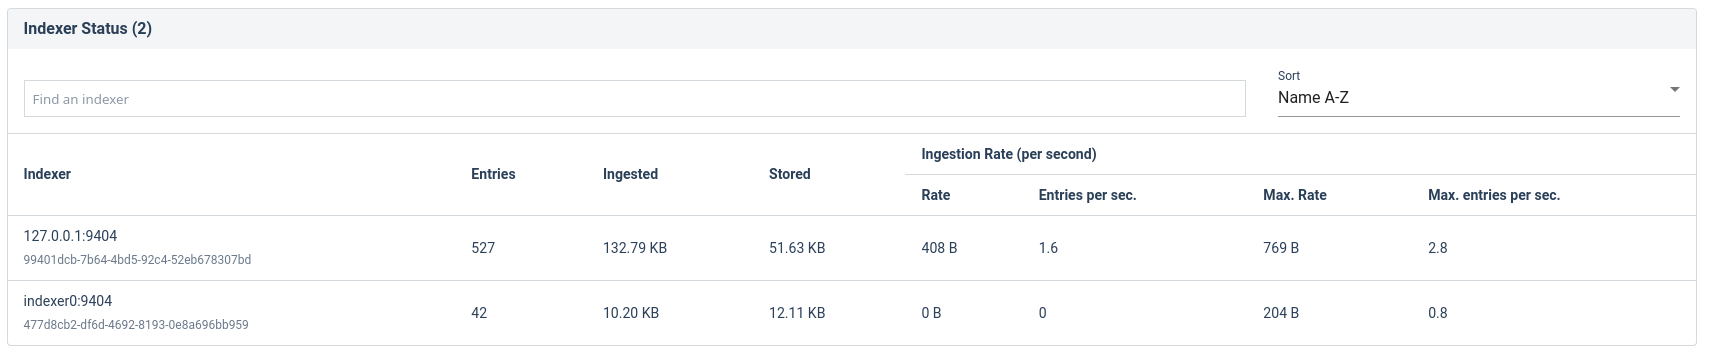
\includegraphics{images/twoindexers.png}
	\caption{Two indexers}
	\label{fig:twoindexers}
\end{figure}

\subsubsection{Lab questions}

\begin{enumerate}
\item
  Why was it necessary to restart the webserver process after updating
  the configuration?
\item
  How would you configure the webserver to \emph{only} communicate with
  the indexer on the indexer0 container, not the local instance?
\end{enumerate}

\section{Configuring Multiple Webservers}
\index{Distributed webservers}\index{Webservers!distributed}\index{Datastore}
Gravwell can use multiple webservers to load-balance user requests.
These webservers must coordinate with each other to manage users,
searches, etc. This coordination is handled through the \textbf{datastore}, a
centralized authority for webserver data.

Setting up a multiple webserver environment comprises configuring the
datastore, pointing the webservers at the datastore, and optionally
installing a load-balancer to balance traffic between the webservers.

The datastore is a separate Gravwell component which must be installed
via self-extracting shell archive available on the Gravwell downloads
page. The datastore can be co-resident with a Gravwell webserver, or it
can run on its own devoted machine. It reads its configuration from
gravwell.conf; for most situations, defaults will be fine, but the following
options are available:

\begin{itemize}
\item
  \code{Datastore-Listen-Address} (default ``'' [all]): specifies which
  IP address the datastore should listen on for connections
\item
  \code{Datastore-Port} (default 9405): specifies the port on which the
  datastore should listen
\item
  Control-Auth: the shared secret by which webservers authenticate to
  the datastore. This must be the same on the datastore and webservers!
\end{itemize}

Webservers must in turn be configured to speak with the datastore using
the following options:

\begin{itemize}
\item
  \code{Datastore}: the address and optional port to connect to the
  datastore, e.g. ``\code{datastore.gravwell.io:9405}''.
\item
  \code{External-Addr}: The address which external systems should use to
  access \emph{this webserver}. It can be an IP address or a DNS name.
  Setting this value allows users on webserver A to view searches on
  webserver B.
\item
  \code{Datastore-Update-Interval} (default 10): how often (in seconds) the
  webserver should check in with the datastore. 10 is a good default.
\end{itemize}

After configuring the webserver's gravwell.conf, restart the webserver
process. It should connect to the datastore and begin synchronizing.
Repeat this for all webservers

\subsection{Hands-on Lab: Configuring multiple webservers}

First, verify that you have the gravwell:webserver, gravwell:indexer, and gravwell:datastore
images available. If not, load them from your images directory as detailed in
Section \ref{sec:load-lab-images}.

Next, we start four containers. One indexer, two webservers, and the
datastore. Note that webserver0 is forwarded to localhost:8080, and
webserver1 is forwarded to localhost:8081:

\begin{Verbatim}[breaklines=true]
docker run --rm -d --name indexer0 gravwell:indexer
docker run --rm -p 8080:80 -d --name webserver0 gravwell:webserver
docker run --rm -p 8081:80 -d --name webserver1 gravwell:webserver
docker run --rm -d --name datastore gravwell:datastore
\end{Verbatim}

Next, we configure each webserver to talk to the datastore. Do the
following for both webserver0 and webserver1, taking care to set the
\code{External-Addr} field properly for each:

Copy the config file to the local system
(e.g. \code{docker exec -it webserver0 vi /opt/gravwell/etc/gravwell.conf})
and add the following in the \code{[Global]} section:

\begin{Verbatim}[breaklines=true]
    Remote-Indexers=net:indexer0:9404
    Datastore=datastore
    External-Addr=webserver0
\end{Verbatim}

Copy the config file back (\code{docker cp /tmp/gravwell.conf webserver:/opt/gravwell/etc/gravwell.conf})
and restart the webserver:

\begin{Verbatim}[breaklines=true]
docker restart webserver0
\end{Verbatim}

\textbf{Make sure you do this for both webserver0 and webserver1!}

Now connect to
\href{http://localhost:8080}{http://localhost:8080} and
\href{http://localhost:8081}{http://localhost:8081} in two separate tabs.
Log in (``admin''/''changeme'') to both,
leaving each open in its own tab.

Open the Groups management screen in the menu bar on both webservers as shown in Figure \ref{fig:webserver-lab-newgroup}.

\begin{figure}
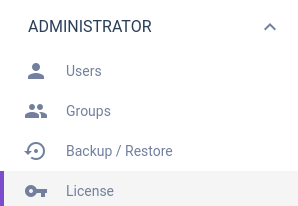
\includegraphics[width=0.4\linewidth]{images/groups-menu.png}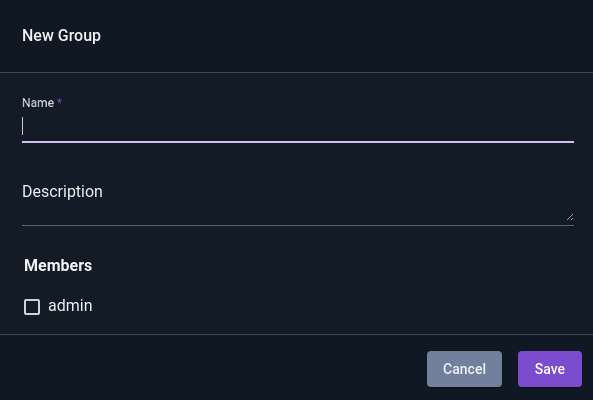
\includegraphics[width=0.5\linewidth]{images/groups-new.png}
\caption{Adding a new group}
\label{fig:webserver-lab-newgroup}
\end{figure}

On one webserver, create a new group; before long, that new group
should be visible on the other webserver's Groups screen too. It may be
necessary to refresh the page.

\subsubsection{Lab questions}

\begin{enumerate}
\item
  Why does it take some seconds for the new group to appear on the
  second webserver? How might this be sped up?
\end{enumerate}

%%%%%%%%%%
% TODO: Kris please update this for the Gravwell load balancer
%%%%%%%%%%
\section{Setting Up a Load-Balancer}
\index{Traefik}\index{Load balancer}
Multiple webservers work well when placed behind a load-balancing
proxy, such as nginx, Traefik, or Gravwell's own load-balancer. 
When using a load-balancer, users simply access
the load-balancer's address (e.g. gravwell.example.org) and are
transparently proxied through to one of the webservers (e.g.
gravwell-webserver-01.example.org).

It is essential that the load balancer be configured with ``sticky''
sessions. This ensures that a given user will be directed to the same
webserver every time.

The Traefik load-balancing proxy has been shown to work well with
Gravwell. The following is a sample configuration which load-balances
between two Gravwell webservers at 10.0.0.1 and 10.0.0.2:

\begin{Verbatim}[breaklines=true]
defaultEntryPoints = ["http", "https"]

[file]

[entryPoints]
    [entryPoints.http]
    address = ":80"
    [entryPoints.https]
    address = ":443"
        [entryPoints.https.tls]
            [[entryPoints.https.tls.certificates]]
            certFile = "traefik.crt"
            keyFile = "traefik.key"

[frontends]
    [frontends.frontend1]
        backend = "backend1"
    [frontends.frontend1.headers]
        SSLRedirect = true
        SSLTemporaryRedirect = true

[backends]
    [backends.backend1]
        [backends.backend1.loadbalancer.stickiness]
        [backends.backend1.servers.server1]
            url="https://10.0.0.1"
        [backends.backend1.servers.server2]
            url="https://10.0.0.2"
\end{Verbatim}
